\chapter{Improving Stress Search Based Testing using Q-Learning and Hybrid Metaheuristic Approach}


\section{Hybrid Approach}

A large number of researchers have recognized the advantages and huge potential of building hybrid metaheuristics. The main motivation for creating hybrid metaheuristics is to exploit the complementary character of different optimization strategies. In fact, choosing an adequate combination of algorithms can be the key to achieving top performance in solving many hard optimization problems \cite{Puchinger2005} \cite{Blum2012}.

The proposed solution makes it possible to create a model that evolves during the test. The proposed solution model uses genetic algorithms, tabu search, and simulated annealing in two different approaches. The study initially investigated the use of these three algorithms. Subsequently, the study will focus in others Population-based and single point search metaheuristics. The first approach uses the three algorithms independently, and the second approach uses the three algorithms collaboratively (hybrid metaheuristic approach).

In the first approach , the algorithms do not share their best individuals among themselves. Each algorithm evolves in a separate way (Fig. \ref{fig:firstaproach}).


\begin{figure}[h]
\centering
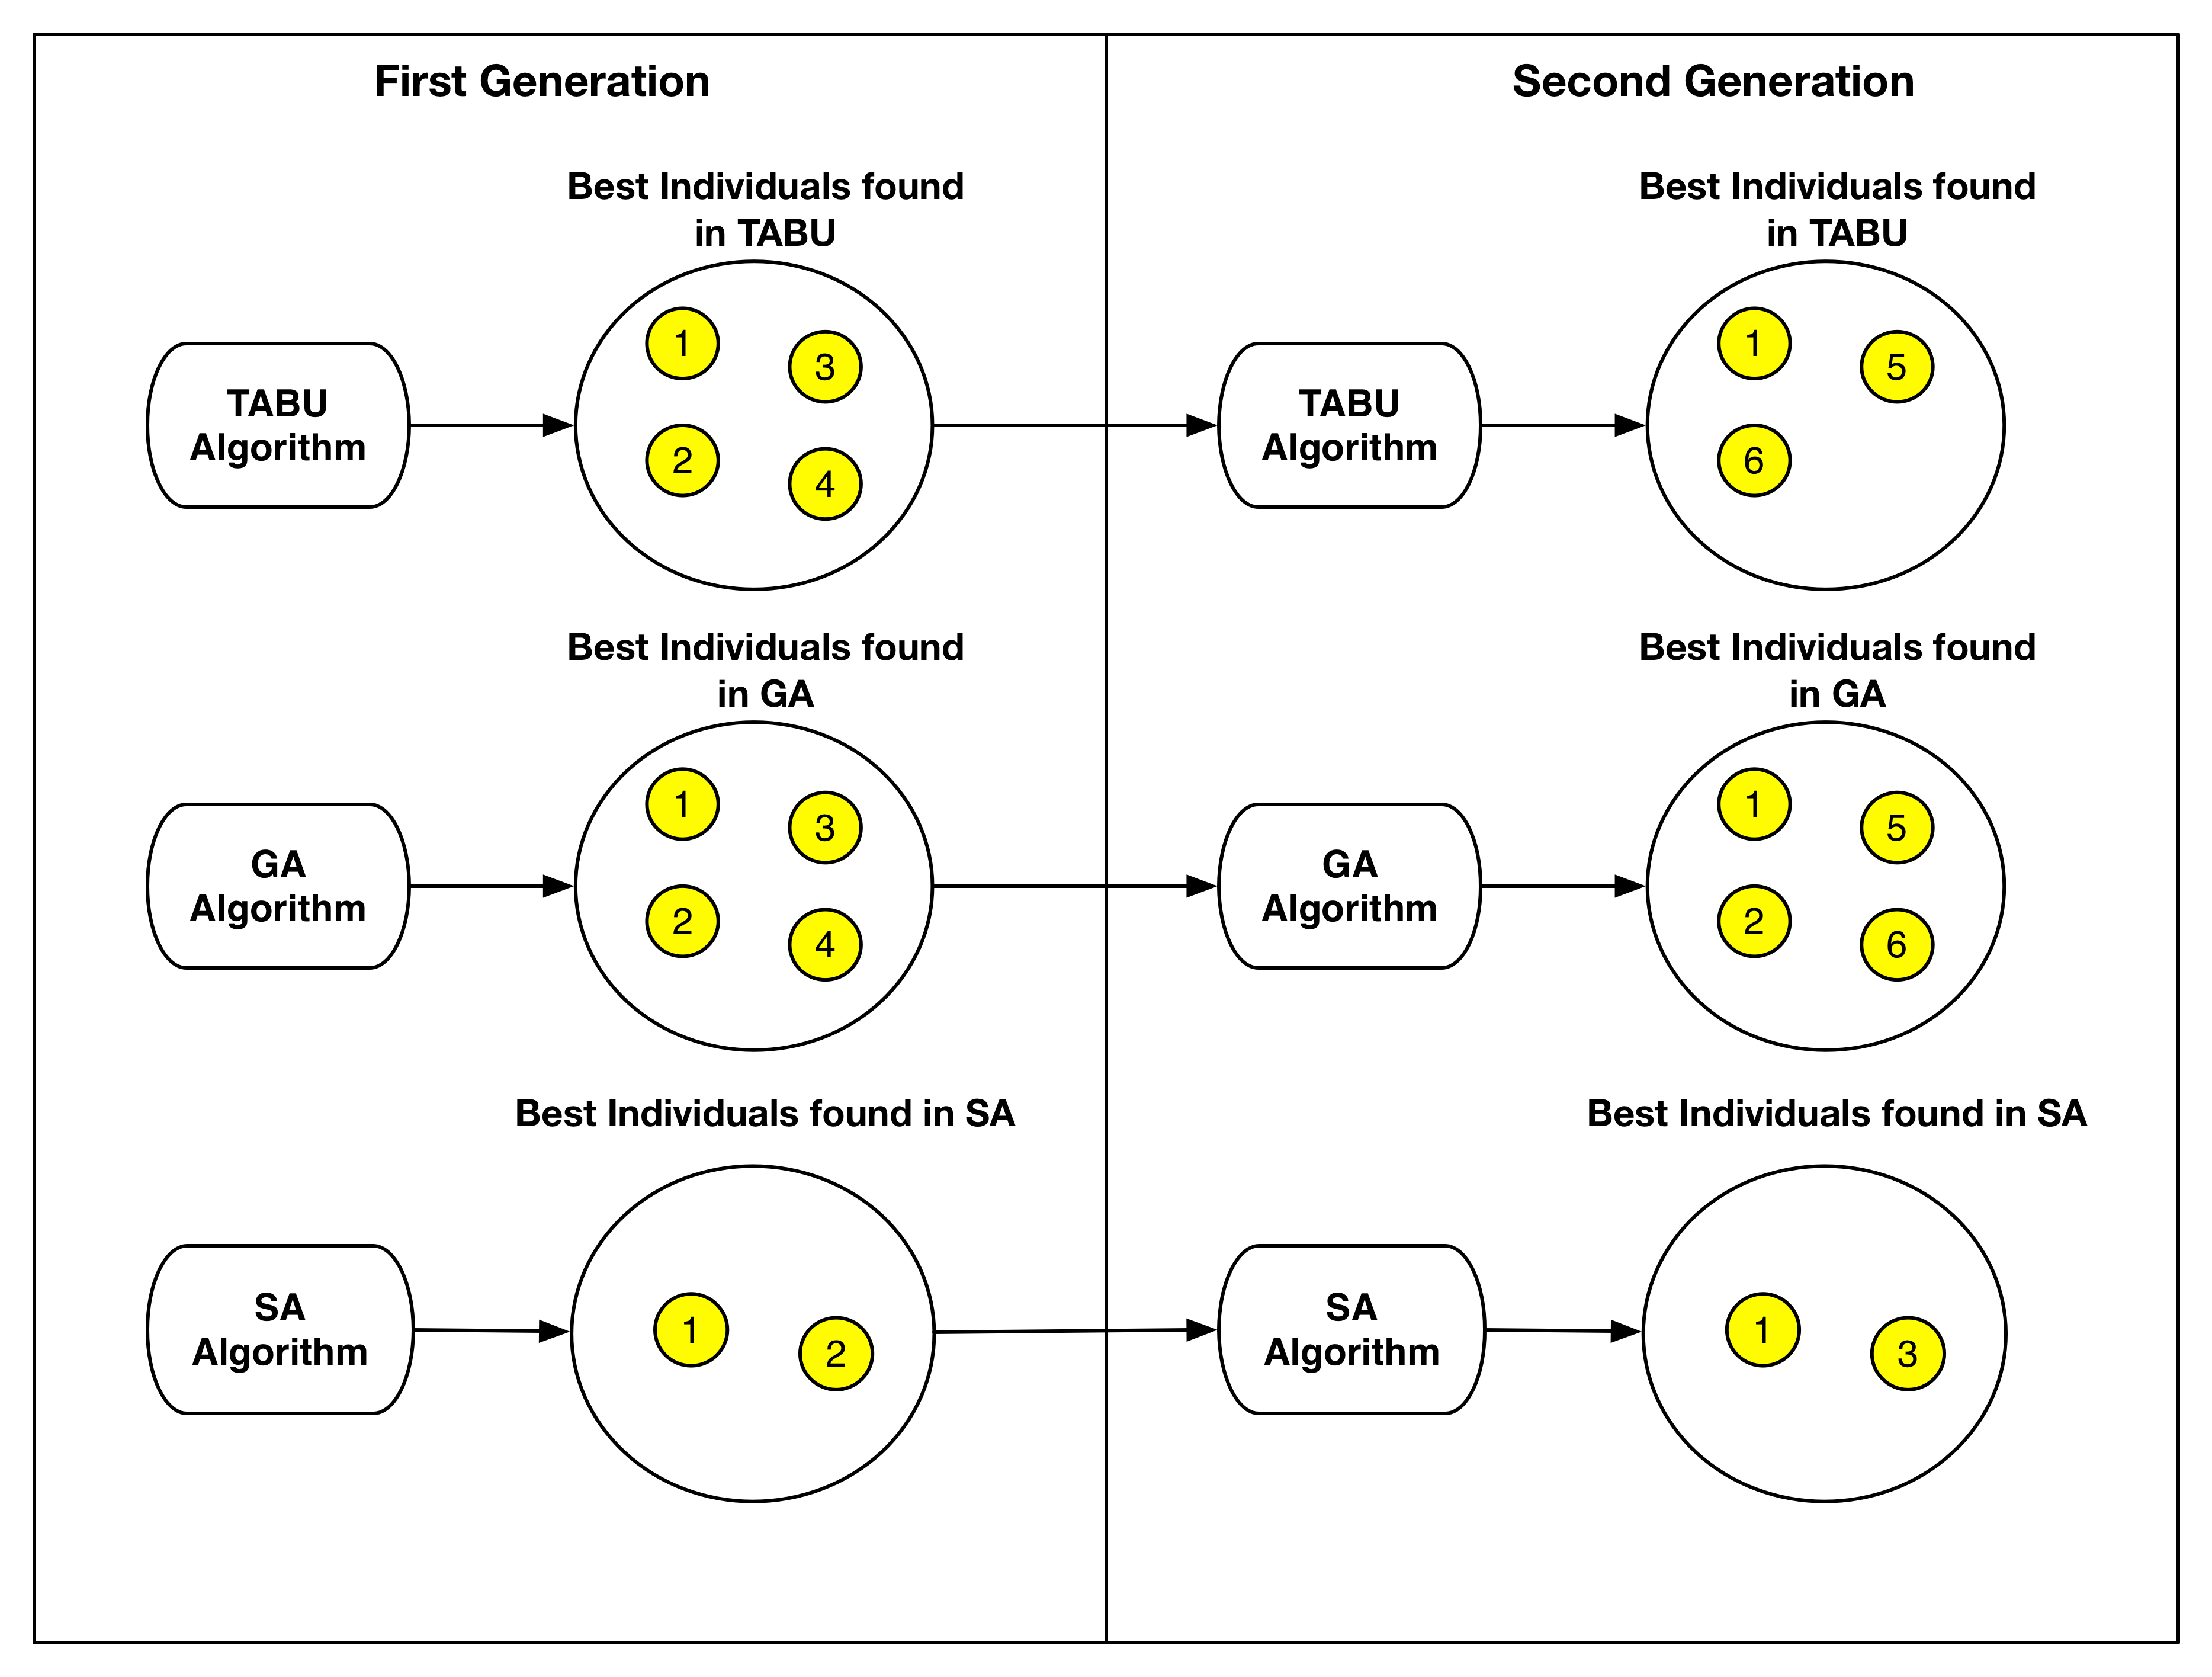
\includegraphics[width=0.7\textwidth]{./images/independ.png}
\caption{Use of the algorithms independently}
\label{fig:firstaproach}
\end{figure}



The second approach uses the algorithms in a collaborative mode (hybrid metaheuristic). In this approach, the three algorithms share their best individuals found (Fig. \ref{fig:secondapproach}). The next subsections present details about the used metaheuristic algorithms (Representation, initial population and fitness function).




\begin{figure}
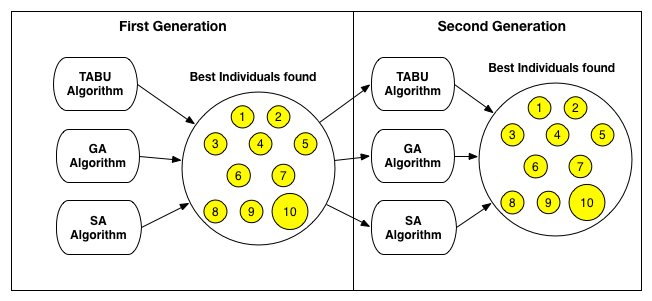
\includegraphics[width=1\textwidth]{./images/collaborative.png}
\caption{Use of the  algorithms collaboratively}
\label{fig:secondapproach}
\end{figure}

\subsection{Representation}

The solution representation is composed by a linear vector with 23 positions. The first position represents the name of an individual. The second position represents the algorithm (genetic algorithm, simulated annealing, or Tabu search) used by the individual. The third position represents the type of test (load, stress, or performance). The next positions represent 10 scenarios and their numbers of users. Each scenario is an atomic operation: the scenario must log into the application, run the task goal, and undo any changes performed, returning the application to its original state.

Fig. \ref{fig:genomarepresentation} presents the solution representation and an example using the crossover operation. In the example, genotype 1 has the Login scenario with 2 users, the Form scenario with 0 users, and the Search scenario with 3 users. Genotype 2 has the Delete scenario with 10 users, the Search scenario with 0 users, and the Include scenario with 5 users. After the crossover operation, we obtain a genotype with the Login scenario with 2 users, the Search scenario with 0 users, and the Include scenario with 5 users.

\begin{figure}[h]
\centering
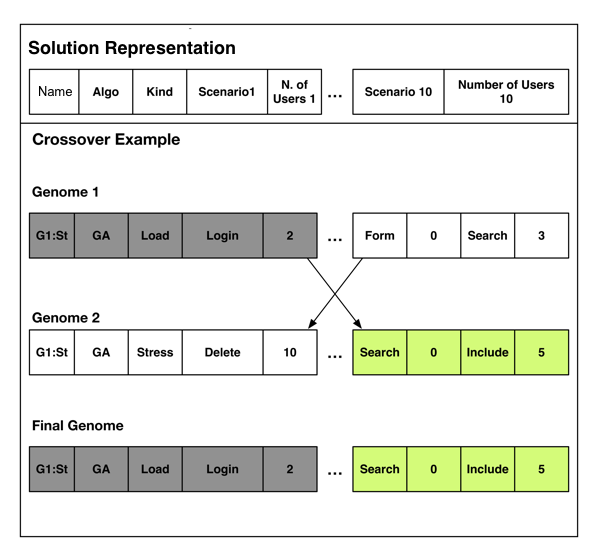
\includegraphics[width=1\textwidth]{./images/genomerepresentation1.png}
\caption{Solution representation and crossover example}
\label{fig:genomarepresentation}
\end{figure}

Fig. \ref{fig:neighbourtaby} shows the strategy used by the proposed solution to obtain the representation of the neighbors for the Tabu search and simulated annealing algorithms. The neighbors are obtained by the modification of a single position (scenario or number of users) in the vector.


\begin{figure}[h]
\centering
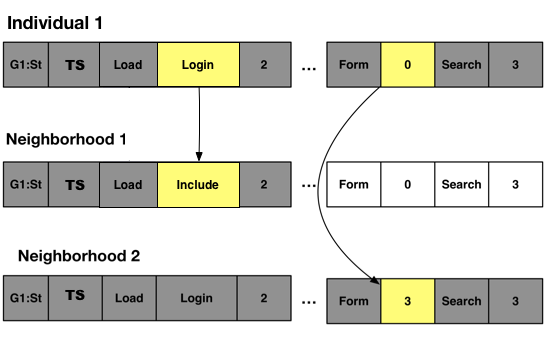
\includegraphics[width=1\textwidth]{./images/neighbor.png}
\caption{Tabu search and simulated annealing neighbor strategy}
\label{fig:neighbourtaby}
\end{figure}


\subsection{Initial population}

The strategy used by the plugin to instantiate the initial population is to generate 50\% of the individuals randomly, and 50\% of the initial population is distributed in three ranges of values:

\begin{itemize}
\item Thirty percent of the maximum allowed users in the test;
\item Sixty percent of the maximum allowed users in the test; and
\item Ninety percent of the maximum allowed users in the test.
\end{itemize}

The percentages relates to the distribution of the users in the initial test scenarios of the solution. For example, in a hypothetical test with 100 users, the solution will create initial test scenarios with 30, 60 and 90 users.

\subsection{Objective (fitness) function}

The proposed solution was designed to be used with independent testing teams in various situations where the teams have no direct access to the environment where the application under test was installed. Therefore, the IAdapter plugin uses a measurement approach to the definition of the fitness function. The fitness function applied to the IAdapter solution is governed by the following equation:

\begin{equation}
\begin{aligned}
fit=90percentileweigth* 90percentiletime\\
+80percentileweigth*80percentiletime\\+
70percentileweigth*70percentiletime+\\
maxResponseWeigth*maxResponseTime+\\
numberOfUsersWeigth*numberOfUsers-penalty
\end{aligned}
\end{equation}

The proposed solution's fitness function uses a series of manually adjustable user-defined weights (90percentileweight, 80percentileweight,  70percentileweight, maxResponseWeight, and numberOfUsersWeight). These weights make it possible to customize the search plugin's functionality. A penalty is applied when an application under test takes a longer time to respond than the level of service. The penalty is calculated by the follow equation:

\begin{equation}
\begin{aligned}
penalty=100 * \Delta \\
\Delta=(t_{Current Response Time} - t_{Maximum Response Time Expected})\\
\end{aligned}
\end{equation}


\section{IAdapter}

IAdapter is a JMeter plugin designed to perform search-based stress tests.  The plugin is available on www.iadapter.org.  The IAdapter plugin implements the solution proposed in Section 5. The next subsections present details about the Apache JMeter tool, the IAdapter Life Cycle and the IAdapter Components. The IAdapter plugin provides three main components: WorkLoadThreadGroup, WorkLoadSaver, and WorkLoadController.

The Fig. \ref{fig:iadapterarchitecture} show the IAdapter architecture. All metaheuristic class implements the interface IAlgorithm. Test scenarios  and test results are stored in a Mysql database. GeneticAlgorithm class uses a framework named JGAP to implement Genetic Algorithms.

\begin{figure}[h]
\center
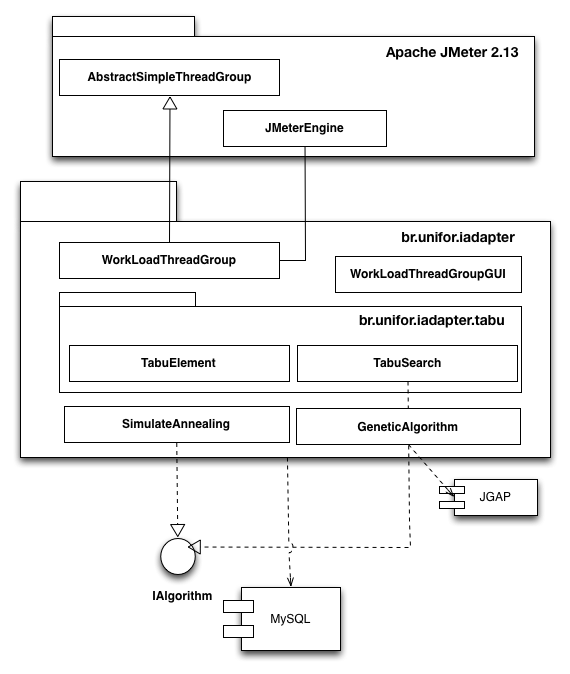
\includegraphics[width=0.8\textwidth]{./images/iadapter1.png}
\caption{IAdapter architecture}
\label{fig:iadapterarchitecture}
\end{figure}

The WorkLoadThreadGroup class is the Load Injection and Test Management modules, responsible to generate the initial population and uses the JMeter Engine to realize requests to server under test. 

\subsection{IAdapter Life Cycle}
 
Fig. \ref{fig:iadapterlifecycle} presents the IAdapter Life Cycle. The main difference between IAdapter and JMeter tool is that the IAdapter provide an automated test execution where the new test scenarios are choosen by the test tool.  In a test with JMeter, the tests scenarios are usually chosen by a test designer.

\begin{figure}[h]
\centering
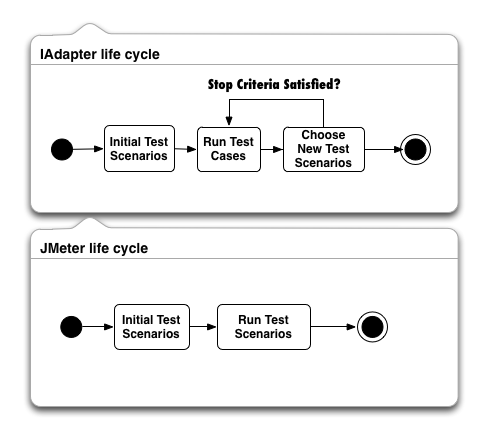
\includegraphics[width=0.8\textwidth]{./images/lifecycle2.png}
\caption{IAdapter life cycle}
\label{fig:iadapterlifecycle}
\end{figure}

\subsection{IAdapter Components}
 
WorkLoadThreadGroup is a component that creates an initial population and configures the algorithms used in IAdapter. Fig. \ref{fig:tela1iadapter} presents the main screen of the WorkLoadThreadGroup component. The component has a name \ding{202}, a set of configuration tabs \ding{203}, a list of individuals by generation \ding{204}, a button to generate an initial population \ding{205}, and a button to export the results \ding{206}.

\begin{figure}[h]
\centering
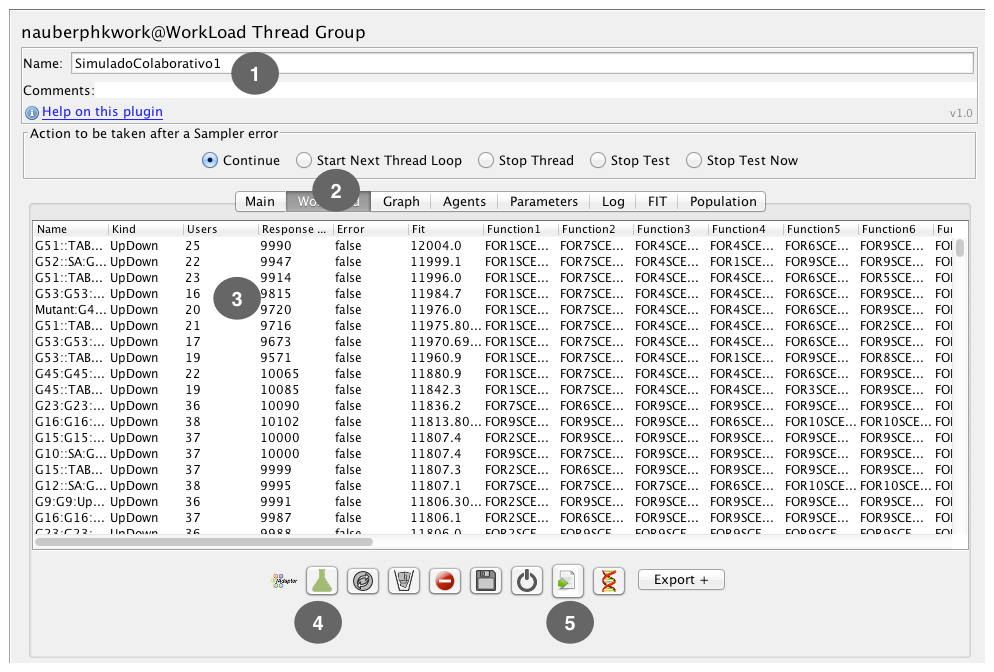
\includegraphics[width=0.8\textwidth]{./images/tela1iadapter.png}
\caption{WorkLoadThreadGroup component}
\label{fig:tela1iadapter}
\end{figure}

WorkLoadThreadGroup component uses the GeneticAlgorithm, TabuSearch and SimulateAnnealing classes.  The WorkLoadSaver component is responsible for saving all data in the database. The operation of the component only requires its inclusion in the test script.

WorkLoadController represents a scenario of the test. All actions necessary to test an application should be included in this component. All instances of the component need to login into the application under test and bring the application back to its original state.


\subsection{IAdapter Testbed Tool}

A Testbed makes possible follow a formalized methodology and reproduce tests for further analysis and comparison. It seems natural that one of the most important parts of a comparison among heuristics is the testbed on which the heuristics are tested. As a result, the testbed should be the first consideration when comparing two metaheuristics \cite{GendreauMichelandPotvin2010}. 

In this section, We devise a new testbed that has the ability to reproduce different types of web workloads.  The proposed solution extends the IAdapter  plugin to create a testbed tool to validade load, performance and stress search based tests approaches \cite{Gois2016}. The IAdapter is a JMeter plugin designed to perform search-based stress tests. 

This new testbed must accomplish three main goals. First, it must reproduce a workload by using an antipattern implementation. Second, it must be able to provide client and server metrics with the aim of being used for web performance evaluation studies. Finally, it is should be extensible, allowing create new test scenarios.

IAdapter Testbed is an open-source facility that provides software tools for search based test research. The testbed tool emulates test scenarios in a controled environment using mock objects and implementing performance antipatterns. 

The testbed tool proposed consists of four main elements. The first element is a emulator module that it is responsible to simulate the antipatterns in a specific context. The second it's a module named test module that it is responsible for use a previous selected metaheuristics and perform a search based test. The third module contains the test scenarios representation. The fourth module it is responsible for provide a service of explore the neighborhood of a given individual. 



\subsubsection{Testbed Architecture}


The Fig. \ref{fig:testbedarch} presents the main architecture of the Testbed solution proposed. The emulator module provides workloads to the Test module.The Test module uses a class loader to find all classes that extends AbstractAlgorithm in the classpath and run all tests for each metaheuristic found. The Test Scenario Representation and Persistent Module provides the scenario representation used by the metaheuristics and persist the testbed results data in a database. Neighborhood provider service is responsible to search neighbors of some individual provided as parameter to the service.

\begin{figure}[h]
\centering
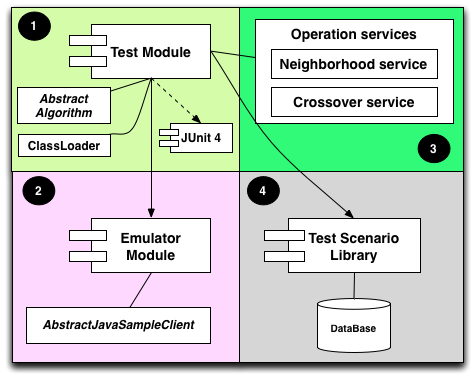
\includegraphics[width=1\textwidth]{./images/testbedarch.png}
\caption{testbed main architecture.}
\label{fig:testbedarch}
\end{figure} 

\begin{figure}[h]
\centering
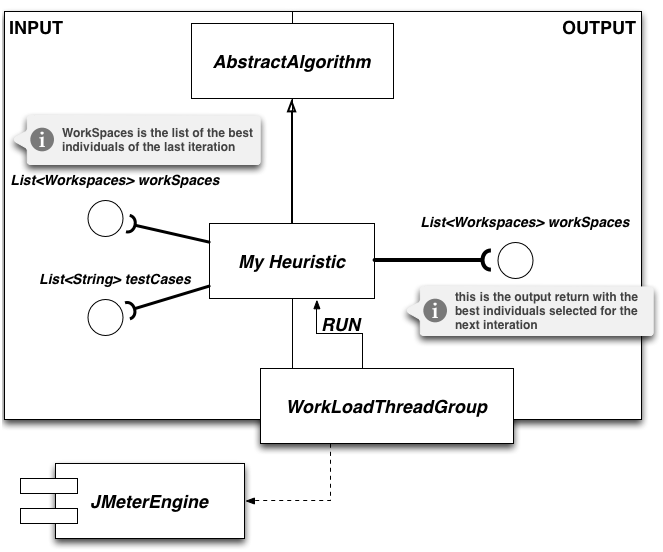
\includegraphics[width=0.8\textwidth]{./images/myheuristic.png}
\caption{Heuristic class diagram.}
\label{fig:heuristicclassdiagram}
\end{figure} 



\subsubsection{Test Module}

The Test Module is responsible for load all classes that extends AbstractAlgorithm in the classpath and perform the tests under the application. The Emulator Module provides successful scenarios and antipatterns implementations. The heuristics are executed in order to select the scenarios with failures or high response times. The Fig. \ref{fig:step1} presents the first feature of Test Module where a initial population it is created and IAdapter with JMeterEngine performs all tests and apply a fitness value to each workload.

\begin{figure}[h]
\begin{minipage}{.5\textwidth}
\centering
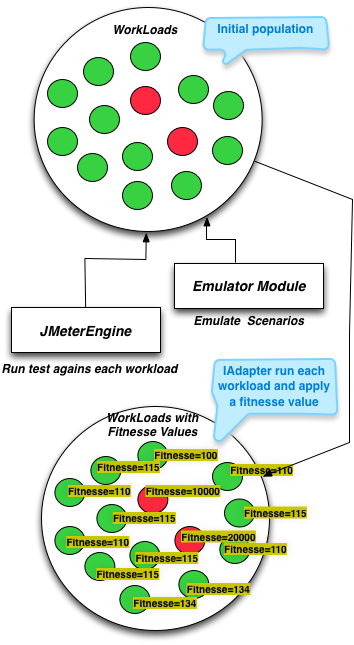
\includegraphics[width=1\textwidth]{./images/step1.png}
\caption{Test Module first feature.}
\label{fig:step1}
\end{minipage}
\begin{minipage}{.5\textwidth}
\centering
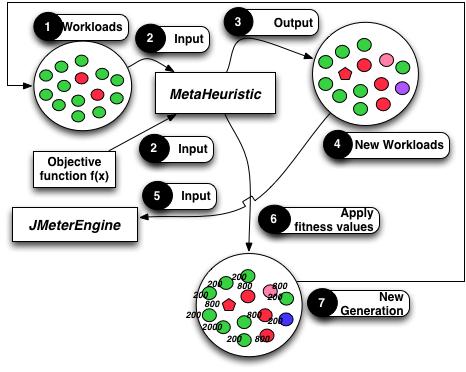
\includegraphics[width=1\textwidth]{./images/step2.png}
\caption{Test Module life cycle.}
\label{fig:step2}
\end{minipage}
\end{figure} 

The Fig. \ref{fig:step2} presents the Test Module life cycle. The life cycle iterate over two steps: The first step apply a metaheurist to select or generate a new set of workloads based on selection criteria. The second step run each workload with the JMeterEngine and obtain a fitness value based on some objective function. The red circles represent the workload that contain errors. The green circles represents the workloads with no errors and low acceptable response time. The testbed tool uses as default objective function the equation:


\begin{equation}
\begin{aligned}
fitness=90percentileweigth* 90percentiletime\\
+80percentileweigth*80percentiletime\\+
70percentileweigth*70percentiletime+\\
maxResponseWeigth*maxResponseTime+\\
numberOfUsersWeigth*numberOfUsers-penalty
\end{aligned}
\end{equation}

The use of presented fitness value by each metaheuristic it's optional. Each Metaheuristic could define your own objective function. The proposed  fitness function uses a series of manually adjustable user-defined weights (90percentileweight, 80percentileweight,  70percentileweight, maxResponseWeight, and numberOfUsersWeight). These weights make it possible to customize the search plugin's functionality. A penalty is applied when an application under test takes a longer time to respond than the level of service. After all these steps the cycle begins until the maximum number of generations it is reached. The Fig. \ref{fig:heuristicclassdiagram} shows the  class diagram for custom and provided heuristics. All heuristic classes extends the class AbstractAlgorithm. The heuristics receives  as input a  list of workspaces and a list of testcases. The workspace represents each individual in the search space.


Each metaheuristic class returns a list of workspaces (the individuals selected to the next generation). The Listing presents the method that performs the search of classes that extends Abstract Algorithm



\subsubsection{Emulator Module}

The Emulator Module is responsible for implement and provide successful scenarios and the most commons performance antipatterns. All classes must extends the AbstractJavaSamplerClient class or use JUnit 4. The AbstractJavaSamplerClient class allows create a JMeter Java Request.  Using JUnit 4, the emulators classes could be called by a JMeter JUnit request. The Fig. \ref{fig:emulator} presents the main features of the emulator module. The module implements 8 test scenarios in its first version.

\begin{figure}[h]
\centering
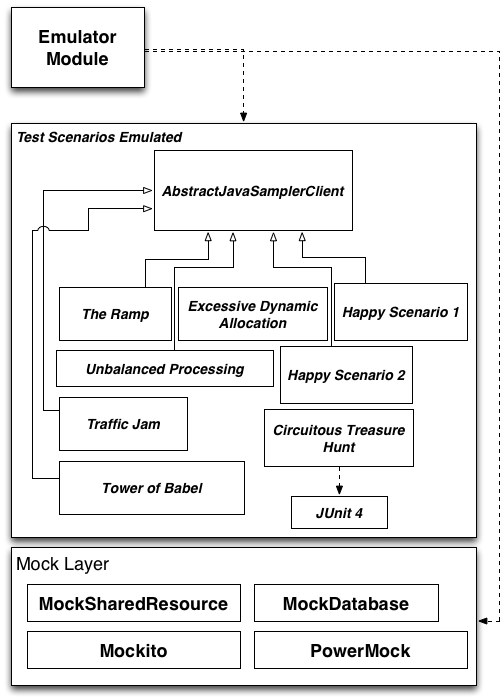
\includegraphics[width=0.7\textwidth]{./images/emulator.png}
\caption{Heuristic class diagram.}
\label{fig:emulator}
\end{figure}  

The Mock Layer provides emulated databases and components to the test scenarios. Each scenario provided by the Emulator Module could be called in JMeter using a Java Request. The algorithm \ref{unbalancedalgorithm} emulates the Unbalanced Processing antipattern. The test scenario C still waiting until A and B scenarios are used by a test.

\begin{algorithm}[H]
  \caption{Unbalanced Processing emulate algorithm}\label{unbalancedalgorithm}
  \begin{algorithmic}[1]
    
    \While{ List of processing scenarios contains A and B }
    \State Processing A and B scenarios
    \EndWhile
    \State Processing scenario C
      
  \end{algorithmic}
\end{algorithm}

The algorithm \ref{rampalgorithm} emulates  the Ramp antipattern. The algorithm increase the response time at each  time that it has been used.

\begin{algorithm}[H]
  \caption{The Ramp emulate algorithm}\label{rampalgorithm}
  \begin{algorithmic}[1]
    \If {count is null}
    \State $count \gets 0  $
    \EndIf
    \State sleep(100* count)
    \State $count \gets count +1  $     
  \end{algorithmic}
\end{algorithm}


The algorithm \ref{excessivedynamicallocation} implements the Excessive Dynamic Allocation antipattern. The algorithm creates a connection with a emulated database, uses the connection and finally the connection.

\begin{algorithm}[H]
  \caption{Excessive Dynamic Allocation emulate algorithm}\label{excessivedynamicallocation}
  \begin{algorithmic}[1]
    
    \For{\textbf{each} request}
        \For{int i=0 to 1000}
        \State Create a connection to a database
        \State Use the connection
        \State Destroy the created connection     
        \EndFor
    \EndFor
      
  \end{algorithmic}
\end{algorithm}

The algorithm \ref{happyscenario1} presents the Happy Scenario 1. The response time increases for every 10 users.

\begin{algorithm}[H]
  \caption{Happy Scenario 1 emulate algorithm}\label{happyscenario1}
  \begin{algorithmic}[1]
    \State sleep(2*users)   
  \end{algorithmic}
\end{algorithm}

\begin{algorithm}[H]
  \caption{Happy Scenario 2 emulate algorithm}\label{happyscenario2}
  \begin{algorithmic}[1]
    \State sleep(3*users)   
  \end{algorithmic}
\end{algorithm}

A further 4 algorithms were developed for the scenarios  Circuitous Treasure Hunt, Happy Scenario 2, Traffic Jam and Tower of Babel.

